\documentclass[tikz,border=8pt]{standalone}
\usepackage[T1]{fontenc}
\usepackage[scaled=0.88]{helvet}
\usepackage{amsmath,amssymb}
\usepackage{tikz}
\usetikzlibrary{arrows.meta,positioning,shapes.geometric,calc}

\begin{document}
\sffamily
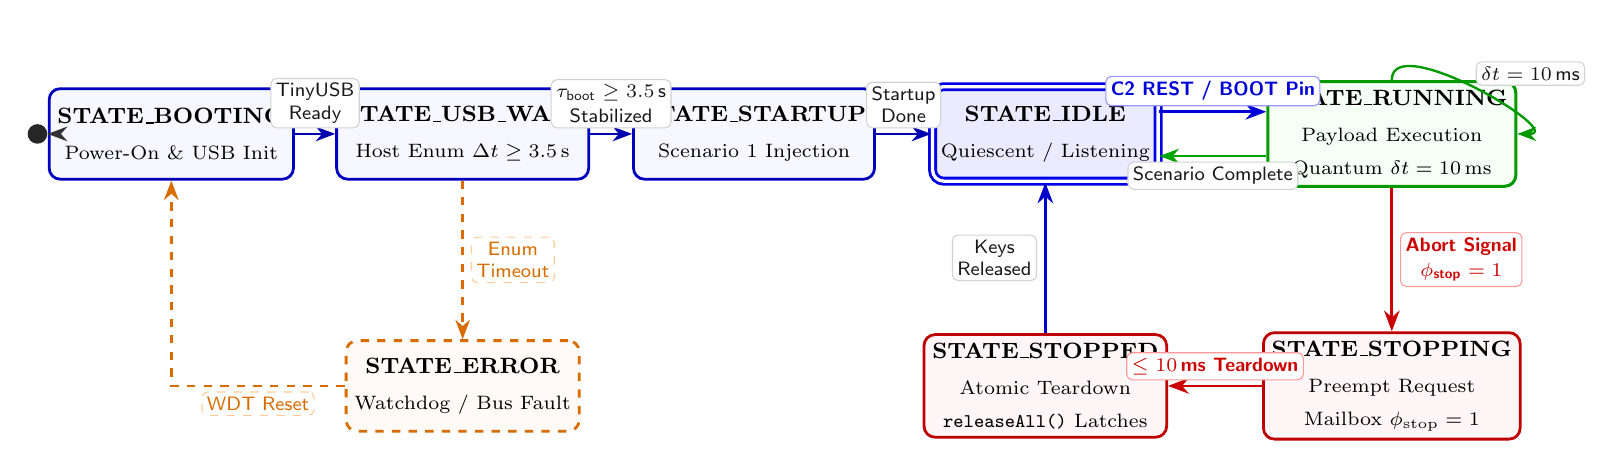
\begin{tikzpicture}[
    >=Stealth,
    font=\small,
    % Standard Operational State
    st_norm/.style={
        rectangle,
        rounded corners=4pt,
        draw=blue!75!black,
        line width=1.0pt,
        fill=blue!3!white,
        minimum width=2.5cm,
        minimum height=1.15cm,
        inner sep=3pt,
        align=center
    },
    % Idle State (Double Border Hub)
    st_idle/.style={
        rectangle,
        rounded corners=4pt,
        draw=blue!90!black,
        double,
        double distance=1.2pt,
        line width=1.0pt,
        fill=blue!8!white,
        minimum width=2.6cm,
        minimum height=1.20cm,
        inner sep=3pt,
        align=center
    },
    % Active Running State
    st_run/.style={
        rectangle,
        rounded corners=4pt,
        draw=green!60!black,
        line width=1.1pt,
        fill=green!4!white,
        minimum width=2.6cm,
        minimum height=1.20cm,
        inner sep=3pt,
        align=center
    },
    % Preempt / Stop States
    st_stop/.style={
        rectangle,
        rounded corners=4pt,
        draw=red!75!black,
        line width=1.0pt,
        fill=red!3!white,
        minimum width=2.5cm,
        minimum height=1.15cm,
        inner sep=3pt,
        align=center
    },
    % Error State
    st_err/.style={
        rectangle,
        rounded corners=4pt,
        draw=orange!85!black,
        line width=1.0pt,
        dashed,
        fill=orange!4!white,
        minimum width=2.5cm,
        minimum height=1.15cm,
        inner sep=3pt,
        align=center
    },
    % Badges
    badge/.style={
        font=\sffamily\scriptsize,
        fill=white,
        draw=gray!35,
        line width=0.4pt,
        rounded corners=2pt,
        inner sep=1.8pt,
        align=center,
        text=black!90
    },
    badge_blue/.style={
        font=\sffamily\scriptsize\bfseries,
        fill=white,
        draw=blue!40,
        line width=0.4pt,
        rounded corners=2pt,
        inner sep=1.8pt,
        align=center,
        text=blue!85!black
    },
    badge_red/.style={
        font=\sffamily\scriptsize\bfseries,
        fill=white,
        draw=red!40,
        line width=0.4pt,
        rounded corners=2pt,
        inner sep=1.8pt,
        align=center,
        text=red!80!black
    },
    badge_amber/.style={
        font=\sffamily\scriptsize,
        fill=white,
        draw=orange!40,
        line width=0.4pt,
        rounded corners=2pt,
        inner sep=1.8pt,
        align=center,
        text=orange!85!black
    }
]

% Start Token
\node[circle, fill=black!85, inner sep=2.5pt] (start) at (0.0, 1.6) {};

% ==============================================================================
% TOP ROW: Main Initialization & Execution Pipeline (y = 1.6)
% ==============================================================================
\node[st_norm] (boot)    at (1.7, 1.6)  {\textbf{\footnotesize STATE\_BOOTING}\\[2pt]\scriptsize Power-On \& USB Init};
\node[st_norm] (usbwait) at (5.4, 1.6)  {\textbf{\footnotesize STATE\_USB\_WAIT}\\[2pt]\scriptsize Host Enum $\Delta t \ge 3.5$\,s};
\node[st_norm] (startup) at (9.1, 1.6)  {\textbf{\footnotesize STATE\_STARTUP}\\[2pt]\scriptsize Scenario 1 Injection};
\node[st_idle] (idle)    at (12.8, 1.6) {\textbf{\footnotesize STATE\_IDLE}\\[2pt]\scriptsize Quiescent / Listening};
\node[st_run]  (running) at (17.2, 1.6) {\textbf{\footnotesize STATE\_RUNNING}\\[2pt]\scriptsize Payload Execution\\[1pt]\scriptsize Quantum $\delta t = 10$\,ms};

% ==============================================================================
% BOTTOM ROW: Fault Recovery & Preemption Teardown Loop (y = -1.6)
% ==============================================================================
\node[st_err]  (error)    at (5.4, -1.6)  {\textbf{\footnotesize STATE\_ERROR}\\[2pt]\scriptsize Watchdog / Bus Fault};
\node[st_stop] (stopped)  at (12.8, -1.6) {\textbf{\footnotesize STATE\_STOPPED}\\[2pt]\scriptsize Atomic Teardown\\[1pt]\scriptsize \texttt{releaseAll()} Latches};
\node[st_stop] (stopping) at (17.2, -1.6) {\textbf{\footnotesize STATE\_STOPPING}\\[2pt]\scriptsize Preempt Request\\[1pt]\scriptsize Mailbox $\phi_{\text{stop}}=1$};

% ==============================================================================
% TRANSITIONS - 100% ORTHOGONAL, ZERO DIAGONALS
% ==============================================================================

% 1. Start -> Booting
\draw[->, line width=0.9pt, draw=black!80] (start) -- (boot);

% 2. Booting -> USB Wait
\draw[->, line width=0.9pt, draw=blue!70!black] (boot) -- node[above=2pt, badge] {TinyUSB\\Ready} (usbwait);

% 3. USB Wait -> Startup
\draw[->, line width=0.9pt, draw=blue!70!black] (usbwait) -- node[above=2pt, badge] {$\tau_{\text{boot}} \ge 3.5$\,s\\[1pt]Stabilized} (startup);

% 4. Startup -> Idle
\draw[->, line width=0.9pt, draw=blue!70!black] (startup) -- node[above=2pt, badge] {Startup\\Done} (idle);

% 5. Idle -> Running (Trigger)
\draw[->, line width=1.0pt, draw=blue!85!black] ([yshift=8pt]idle.east) -- node[above=2pt, badge_blue] {C2 REST / BOOT Pin} ([yshift=8pt]running.west);

% 6. Running -> Idle (Normal Completion)
\draw[->, line width=0.9pt, draw=green!65!black] ([yshift=-8pt]running.west) -- node[below=2pt, badge] {Scenario Complete} ([yshift=-8pt]idle.east);

% 7. Cooperative Quantum Slicing Self-Loop on RUNNING
\draw[->, line width=0.85pt, draw=green!60!black] (running.north) .. controls +(up:0.65cm) and +(right:0.65cm) .. node[above right=1pt, badge] {$\delta t = 10$\,ms} (running.east);

% 8. Running -> Stopping (Preempt / Abort) - Straight Vertical Down!
\draw[->, line width=1.0pt, draw=red!80!black] (running.south) -- node[right=3pt, badge_red] {Abort Signal\\[1pt]$\phi_{\text{stop}}=1$} (stopping.north);

% 9. Stopping -> Stopped (Atomic Teardown) - Straight Horizontal Left!
\draw[->, line width=1.0pt, draw=red!80!black] (stopping.west) -- node[above=2pt, badge_red] {$\le 10$\,ms Teardown} (stopped.east);

% 10. Stopped -> Idle (Return to Quiescent) - Straight Vertical Up!
\draw[->, line width=1.0pt, draw=blue!80!black] (stopped.north) -- node[left=3pt, badge] {Keys\\Released} (idle.south);

% 11. USB Wait -> Error (Timeout Fault) - Straight Vertical Down!
\draw[->, line width=0.9pt, dashed, draw=orange!85!black] (usbwait.south) -- node[right=3pt, badge_amber] {Enum\\Timeout} (error.north);

% 12. Error -> Booting (WDT Reset Recovery) - Orthogonal Corner!
\draw[->, line width=0.9pt, dashed, draw=orange!85!black] (error.west) -| node[pos=0.25, below=2pt, badge_amber] {WDT Reset} (boot.south);

\end{tikzpicture}
\end{document}
